%----------------------------------------------------------------
%
%  File    :  integration.tex
%
%  Authors :  David Lechner, FH Campus Wien, Austria
%
%  Created :  10 March 2020
%
%  Changed :  10 March 2020
%
%----------------------------------------------------------------


\chapter{Integration ins Fahrzeug}
\label{chap:car_integration}

In diesem Kapitel wird gezeigt, wie das System zur Erkennung des Lenkers prototypisch in ein Fahrzeug integriert werden kann. Die Anwendung soll insbesondere folgende Aufgabe erfüllen:

\begin{description}
    \item[] Aus einem Set von vier bekannten Fahrerprofilen soll die aktuell fahrende Person zugeordnet werden können.
\end{description}

Laut Statistik Austria hat die durchschnittliche österreichische Familie 1,68 Kinder (Stand 2018) \cite{Stat2018}. Aufgerundet besteht sie daher aus vier Personen und deshalb die Anzahl der Fahrerprofile.

Die Anforderung zielt speziell auf konkrete Anwendungsfälle, welche zum Teil bereits in der Einleitung erläutert wurden, ab. Mit den Erkenntnissen lassen sich Maßnahmen umsetzten, um beispielsweise mehr Komfort bieten zu können. Darunter fällt das Einstellen des bevorzugten Radiosenders oder das Anzeigen der letzten Ziele im Navigationssystem für eine schnellere Auswahl. Andere Möglichkeiten, wie diese Information genutzt werden kann, werden weiters noch im nächsten Kapitel diskutiert.

\section{Systemarchitektur}
\label{sec:architecture}

Das Gesamtsystem kann mit zwei verschiedenen Architekturen umgesetzt werden. Bei beiden Varianten gibt es vier Komponenten. Ausgangspunkt sind die Steuergeräte, die in einem Fahrzeug über den CAN-Bus vernetzt sind. Eine zentrale Logikeinheit, die \textit{Car Connectivity Unit} (CCU), zeichnet die CAN-Nachrichten auf und verarbeitet diese. Sie ist nicht Teil eines Serienfahrzeuges und muss nachgerüstet werden. Beim ersten Ansatz überträgt die CCU alle CAN-Daten zu einem \textit{Cloud}-Service, wo sie von einem bereits trainierten \textit{Machine Learning Model} klassifiziert werden. Aufgrund dessen liegen die Profile der autorisierten Lenker eines Fahrzeugs auch in der \textit{Cloud}. Das Ergebnis um welche Fahrerin es sich handelt, wird entweder über einen Email- oder SMS-Provider zurück ins Auto oder zum Fahrzeughalter gesendet. Beim zweiten Ansatz wird alles auf der CCU durchgeführt. Sie trainiert ein Model mit den Fahrerprofilen, liest CAN-Nachrichten mit, führt die Klassifizierung durch und versendet das Ergebnis. Die Abbildungen \ref{fig:arch1} und \ref{fig:arch2} bilden die Ansätze ab.

\begin{figure}
    \centering
    \begin{subfigure}[c]{0.48\textwidth}
        \centering
        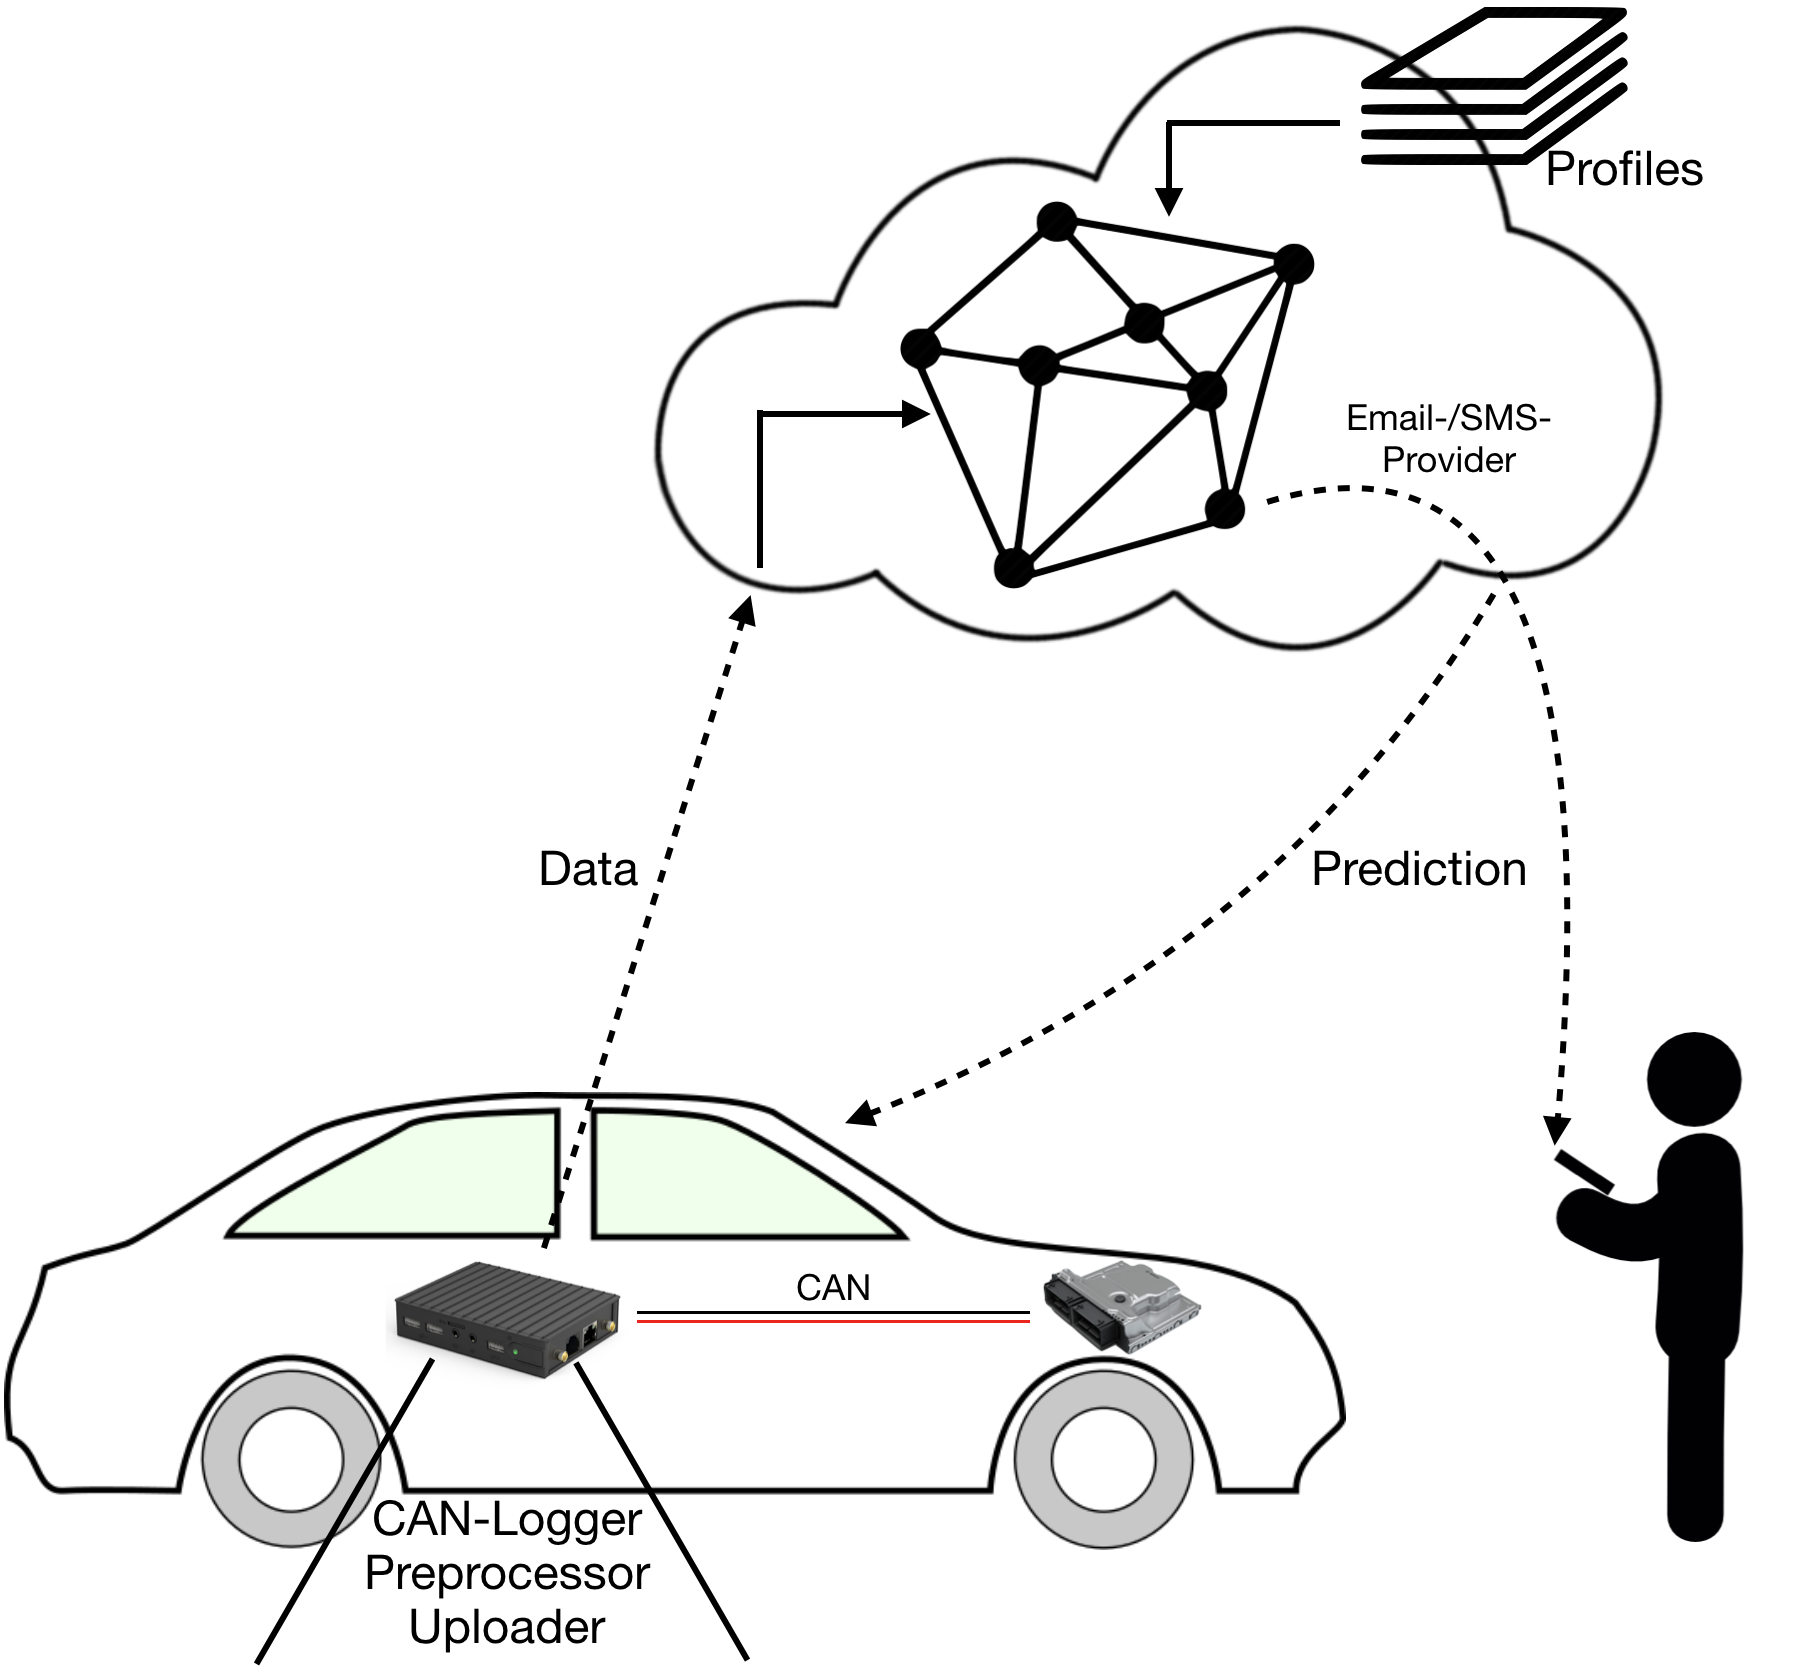
\includegraphics[width=\textwidth]{images/arch_type1.png}
        \subcaption{Architektur 1}
        \label{fig:arch1}
    \end{subfigure}
    \hfill
    \begin{subfigure}[c]{0.48\textwidth}
        \centering
        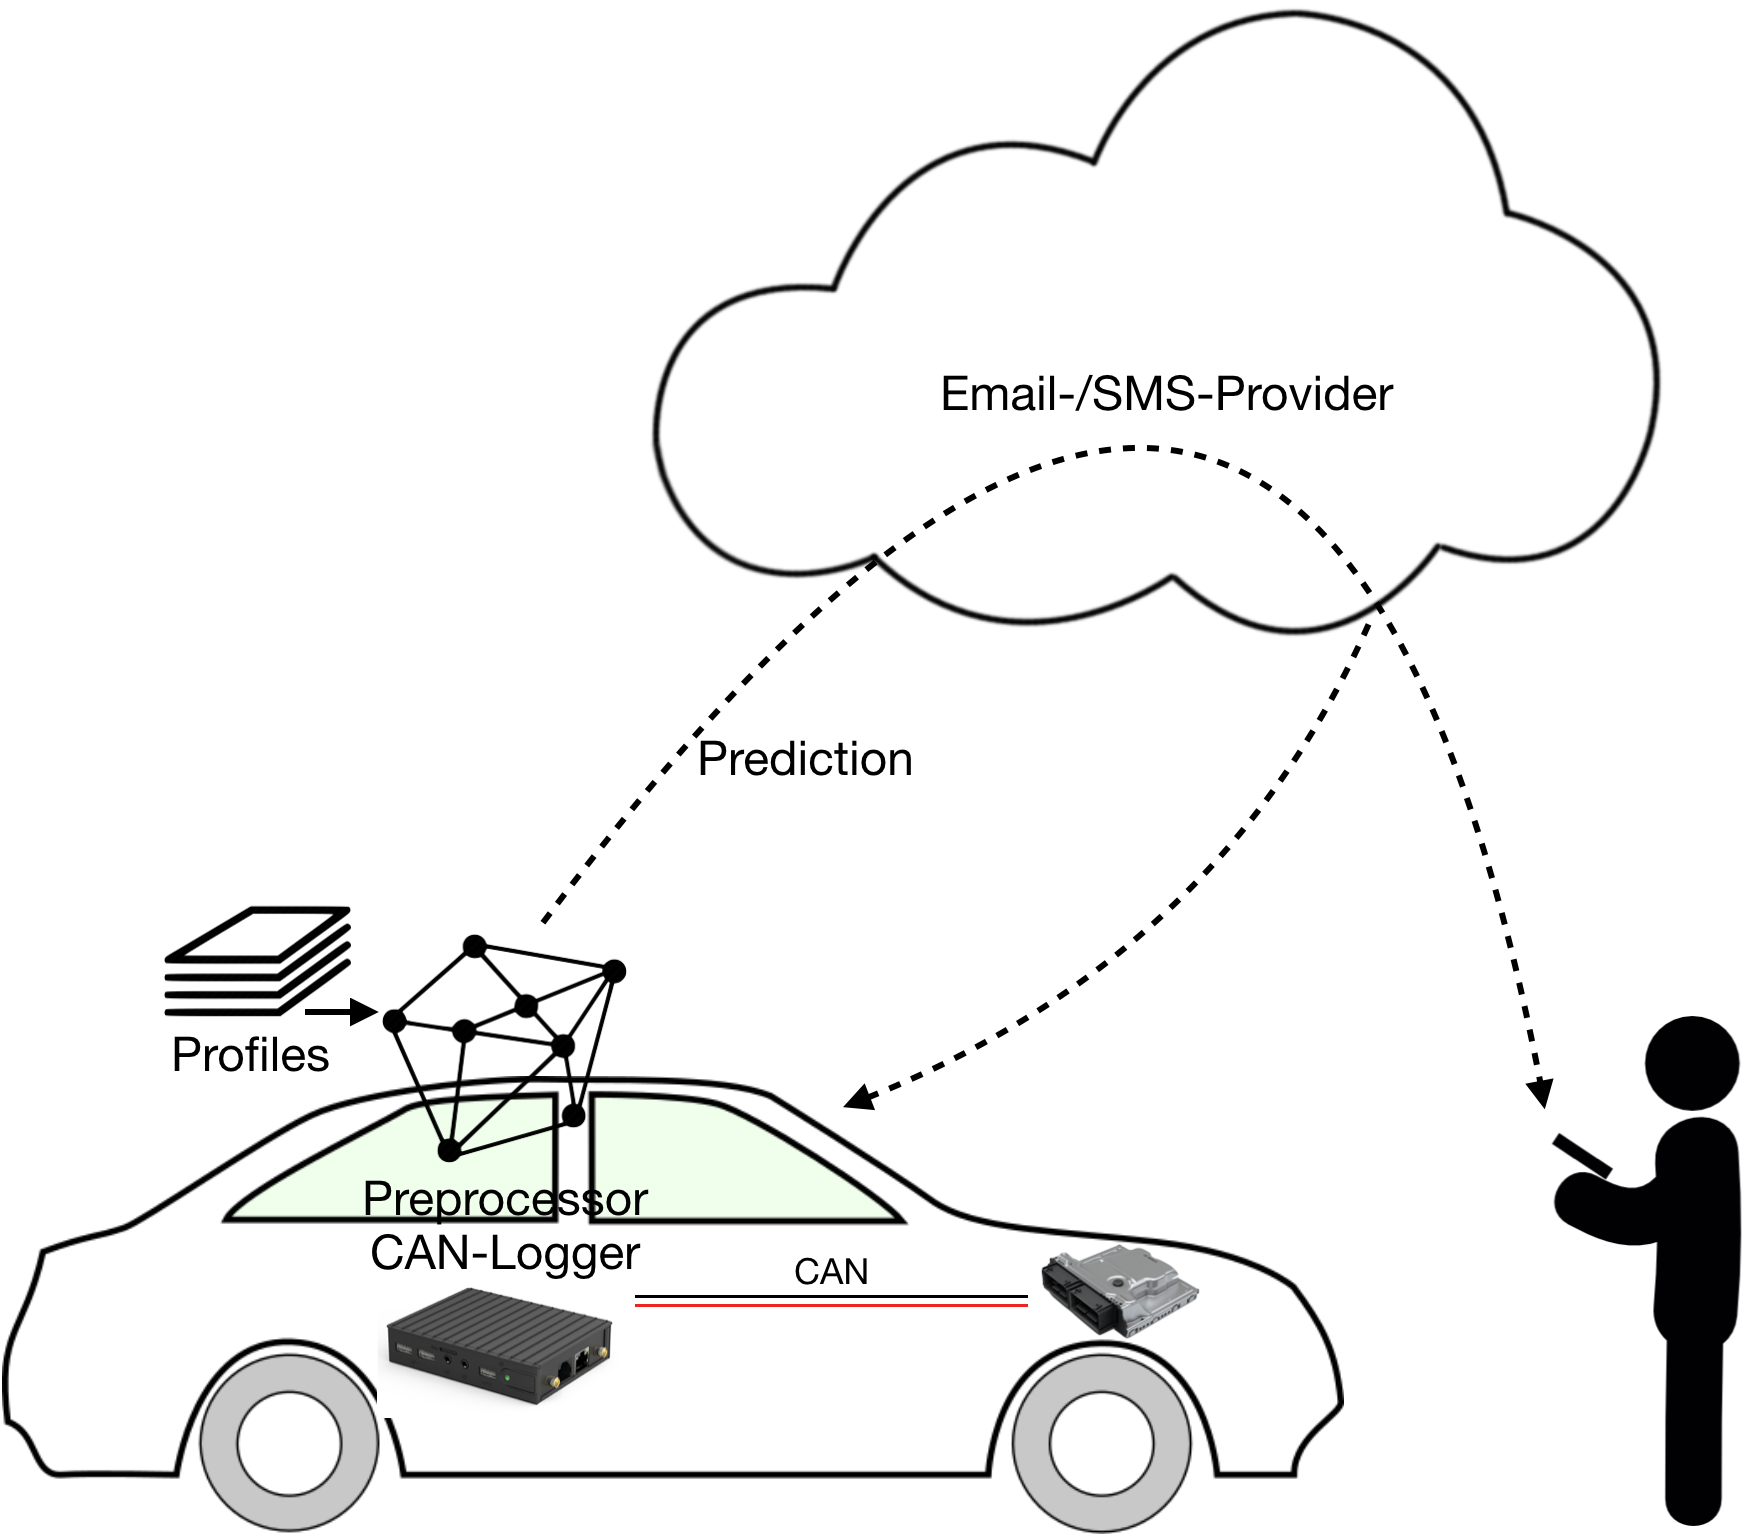
\includegraphics[width=\textwidth]{images/arch_type2.png}
        \subcaption{Architektur 2}
        \label{fig:arch2}
    \end{subfigure}
    \caption{Mögliche Architekturen}
\end{figure}

Der Hauptunterschied bei beiden liegt darin, wo jegliche \textit{Machine Learning} Anwendungen laufen. Dies zieht jedoch eine Reihe von Konsequenzen mit sich. In erster Linie wird dem System Komplexität genommen, wenn Komponenten wegfallen. In diesem Fall ist es das ML-\textit{Cloud}-Service. Die CCU muss im zweiten Ansatz keine Verbindung in die \textit{Cloud} aufbauen und Daten übertragen. Da es sich dabei mitunter um sensible Daten handelt, fallen zudem alle Anforderungen bezüglich CIA - \textit{Confidentiality}, \textit{Integrity}, \textit{Authenticity} - weg. Der Kommunikationskanal müsste sonst gegen ein unerlaubtes Abgreifen der Daten verschlüsselt, gegen eine Verfälschung integritätsgeschützt und authentifiziert sein, damit potentielle Angreifer keine Daten einspeisen können. Die ersten beiden Kriterien können einfach mit dem Einsatz von \textit{HTTPS} sichergestellt werden. Hierzu muss lediglich ein entsprechendes Zertifikat am Server installiert sein, welches für den Daten-Upload verwendet wird. Für die Gewährleistung der Authentizität können zum Beispiel Client-Zertifikate eingesetzt werden. Dafür ist eine eigene \textit{Public Key Infrastructure} (PKI) nötig, um die Zertifikate auf den CCUs zu verwalten.

Ein weiterer Nachteil des zweiten Ansatzes ist, dass Übertragungs- und Verbindungsabbrüche korrekt behandelt werden müssen. Dazu zählt die Verifizierung eines erfolgreichen Uploads, die Wiederaufnahme eines Abbruchs und die Sicherstellung, dass nichts mehrfach hochgeladen wird. Nicht nur die Kommunikation zwischen der \textit{Connectivity Unit} und der \textit{Cloud} erfordert Maßnahmen gegen \textit{Security Threats}, sondern auch die \textit{Cloud} an sich. Sie muss mit einer \textit{Firewall} abgesichert, ein unerlaubter Austausch und Verfälschung der Profile verhindert werden. Wie bereits in den Grundlagen \ref{sec:edge_computing} \textit{Edge Computing} erläutert, hat die Wahl der Architektur auch eine Auswirkung auf den Datenschutz. Bleiben die Daten nur offline am Gerät, muss deutlich weniger beachtet werden, als wenn sie in die \textit{Cloud} hochgeladen werden.

Der zweite Ansatz hat aber auch Nachteile. So ist beispielsweise die Verteilung von Updates schwieriger, da diese auf jeder CCU eingespielt werden müssen und nicht nur zentral in der \textit{Cloud}. Es könnte mitunter auch zu Performance-Problemen kommen, falls das \textit{Embedded-Device} zu wenig Ressourcen für \textit{Machine Learning} Anwendungen hat. Im Ansatz 1 kann durch eine einfache und schnelle Skalierung der CPUs/GPUs beziehungsweise des Arbeitsspeichers der IaaS-Provider die Leistung an die Anforderungen angepasst werden. Auch die Administration der Fahrerprofile wie zum Beispiel das Hinzufügen oder Löschen lässt sich einfacher gestalten, wenn sie auf der \textit{Cloud} abliegen. Es gibt noch mehr Punkte, welche in die Entscheidung der zu implementierenden Architektur miteinfließen. Darunter fällt das Logging, Monitoring, erweitertes \textit{Security}-Konzept oder wie das gesamte System auf viele Fahrzeuge skaliert werden kann. Da es jedoch nur prototypisch für ein einziges Auto realisiert wird, werden diese Punkte nicht näher erläutert.

Der zweite Ansatz ist aufgrund der überwiegenden Vorteile, vor allem weil die Komplexität durch die Kommunikation mit der \textit{Cloud} wegfällt, zu bevorzugen und wird daher in weiterer Folge umgesetzt.

\section{Car Connectivity Unit}
\label{sec:ccu}

Der zentrale Baustein des Systems zur Identifizierung eines Fahrers ist die \textit{Car Connectivity Unit}, welche im Auto verbaut wird. In der Architekturbeschreibung wurde schon auf ihre Funktionen hingewiesen. Daraus lassen sich folgende Hardware-Anforderungen für das Device extrahieren:

\begin{itemize}
    \item kompakte Bauweise für das automotiv Umfeld
    \item CAN-Interface
    \item ausreichend Ressourcen für \textit{Machine Learning} Anwendungen
    \item LTE Modem
    \item Debug/Flash Schnittstelle
\end{itemize}

Prinzipiell könnte ein \textit{Raspberry-Pi} mit entsprechenden Modulen und einem robusten Gehäuse in Frage kommen. Da jedoch das Unternehmen \textit{Bosch} eine Reihe an dezidierten CCUs im Portfolio hat und bei einer schon viel Know-How vorhanden ist, wird die sogenannte \textit{Automotive Linux Edge Node} (ALEN) eingesetzt. Ursprünglich ist das israelische Unternehmen \textit{CompuLab} \footnote{\url{https://www.compulab.com/products/iot-gateways/}} der Hersteller des Geräts und \textit{Bosch} passt es an Automotive-Bedingungen an. Darunter fällt die Verstärkung des Gehäuses, das Hinzufügen einer CAN-Schnittstelle (RJ11-Buchse) sowie der Austausch des LTE-Moduls. Des Weiteren verfügt die ALEN über vier USB-Ports, eine serielle Schnittstelle über Micro-USB, ein WiFi Modul, zwei Gigabit Ethernet-Buchsen, jeweils einen Audio Ein- und Ausgang sowie einen HDMI-Ausgang. Hinzu kommen noch einige GPIOS, I2C, UART und SPI Interfaces. Als Prozessor ist ein 1GHz NXP i.MX 7Dual ARM Cortex-A7 verbaut, 1GB RAM sowie ein 12GB Flash-Speicher. Die Versorgungsspannung beträgt 12V. Die Abbildungen \ref{fig:alen} zeigt die CCU.

\begin{figure}[htbp]
	\centering
    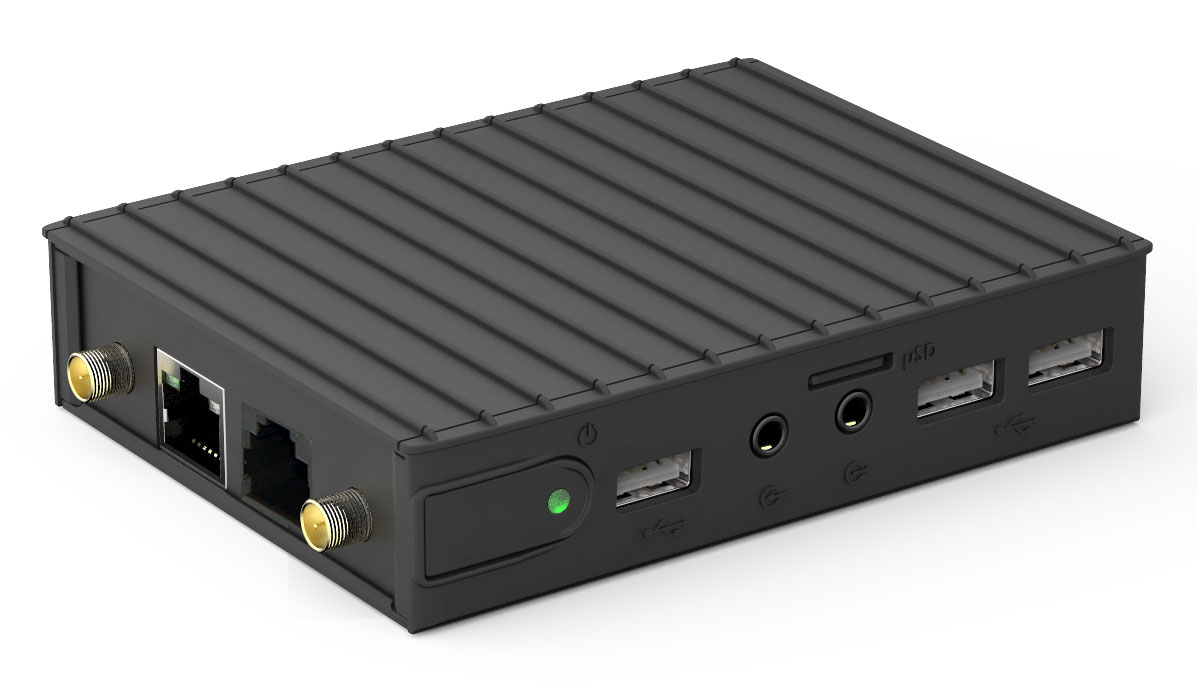
\includegraphics[width=.5\textwidth]{images/alen.jpg}
	\caption{\textit{Automotive Linux Edge Node} (ALEN, Quelle: \url{https://www.compulab.com/products/iot-gateways/})}
	\label{fig:alen}
\end{figure}

Auf der ALEN läuft ein individuelles Linux-System, welches für die Hardware angepasst und mithilfe einer SD-Karte auf das Gerät geladen wird. Zum Erstellen dieser speziellen Linux Distribution wird \textit{Yocto} verwendet.

\subsection{Yocto}
\label{sec:yocto}

\textit{Yocto} \cite{Yocto20} ist ein \textit{Open-Source} Projekt bestehend aus verschiedenen \textit{Templates}, \textit{Tools} und Methoden, um ein Linux-basiertes Betriebssystem für eingebettete Systeme zu bauen. Es wurde 2010 von der \textit{Linux Foundation} ins Leben gerufen und wird seither auch von ihr verwaltet. Die drei Hauptkomponenten sind \textit{BitBake}, \textit{OpenEmbedded-Core} und \textit{Poky}. Ersteres ist die \textit{Build Engine}, ähnlich wie \textit{make} für \textit{C}. Sie interpretiert Konfigurationsdateien und \textit{Recipes} (siehe weiter unten) und führt davon ausgehend Aktionen aus, beispielsweise herunterladen von \textit{Source-Code} oder Binärdateien, konfigurieren und bauen von Applikationen sowie das Dateisystem. Die zweite Komponente ist eine Sammlung aus Basis-\textit{Layer} für einige Hardwarearchitekturen wie zum Beispiel ARM oder MIPS. \textit{Poky} ist sozusagen der Grundstein für jegliches Betriebssystem und vereint alles was dafür benötigt wird.

Jedes \textit{Yocto} Projekt besteht aus mehreren Schichten (\textit{Layer}), wobei die erste eben \textit{Poky} ist. Diese bringt auch den Linux-Kernel mit ein. Die zweite Schicht beinhaltet alle Informationen für die zu verwendete Hardware und wird auch das \textit{Board Support Package} (BSP) genannt. Darunter zählen die Kernel-Konfigurationen, der \textit{Device-Tree} und Treiber. Für die ALEN stellt der Hersteller \textit{Compulab} diese Schicht bereit. Die darüber liegenden \textit{Layer} können weitere Spezifikationen und Modifikationen für das BSP enthalten, wenn z.B. sich die Peripherie geändert hat. Eine Regel der \textit{Yocto-Community} besagt nämlich, dass niemals Basisschichten direkt verändert werden dürfen, sondern nur durch höhere. Dazwischen können noch weitere Schichten liegen, eventuell eine \textit{Security}-Schicht, welche \textit{Recipes} und Konfigurationen für einen sicheren Update-Mechanismus oder \textit{SSH} umfasst. Die letzte Schicht wird dazu verwendet, um Anwender-Software hinzuzufügen, Benutzer anzulegen oder Konfigurationen für Dienste zu ändern.

All diese \textit{Layer} enthalten die angesprochenen \textit{Recipes}, welche Tasks spezifizieren, die wiederum von \textit{BitBake} ausgeführt werden. Im Allgemeinen handelt es sich dabei um Informationen über eine einzelne Applikation. Diese inkludieren meistens den Ort von wo der \textit{Source-Code} bezogen wird (z.B. \textit{GitHub}), spezielle Einstellungen, wie kompiliert wird und wohin die resultierenden Dateien im Zielsystem gespeichert werden. Des Weiteren können auch \textit{Patches} vorhanden sein, die andere \textit{Recipes} anpassen. Sie sind notwendig, wenn ein Pfad geändert werden muss, Kernel-Configs oder neue Dateien hinzukommen. Wird nun über die \textit{Build Engine} ein \textit{Image} gebaut, werden alle \textit{Recipes} nach der Reihe bzw. parallel ausgeführt. Das Ergebnis ist das gesamte \textit{Root-Filesystem} und alle Informationen die für das Booten des Geräts benötigt werden.

Das ist zugleich ein großer Vorteil von \textit{Yocto} \cite{Yocto220}. Beim traditionellen Aufsetzen eines Linux-basierten Systems wird ein standard Betriebssystem installiert und im Nachhinein konfiguriert, neue Softwarepakete installiert usw. Hierbei ist das Zielsystem bereits voll eingerichtet und erfordert keine weiteren Aktionen für den gewünschten Betrieb. Zudem gibt es eine große \textit{Community} rund um \textit{Yocto}, die einerseits das Projekt stets voranbringt und andererseits viel Support bei Problemen liefert. Ein Vorteil ist auch, dass die erforderliche \textit{Toolchain} zum Entwickeln voll enthalten ist und leicht an eigene Bedürfnisse angepasst werden kann. Zusätzlich bietet das \textit{Layer}-Modell Flexibilität und Wiederverwendung der einzelnen Schichten. Soll ein System auf eine andere Hardware portiert werden, braucht nur das \textit{Board Support Package} ausgetauscht werden. Durch die Komplexität ergibt sich unweigerlich eine große Einstiegshürde. Die Lernkurve ist anfangs sehr steil und initial muss viel Zeit aufgewendet werden, um alles Notwendige einsatzfähig zu haben. Nichtsdestotrotz ist \textit{Yocto} bei der Erstellung von hardwareabhängigen Betriebssystemen für \textit{Embeded Systems} und vor allem auch für den IoT Bereich sehr beliebt.

Die unten angeführte Abbildung zeigt die \textit{Layer} für dieses Projekt. Hier ist anzumerken, dass die Namenskonvention den Präfix \textit{meta-} für die \textit{Layer} vorschreibt. Die ersten zwei Schichten bilden die Basis mit dem Linux-Kernel. \textit{Freescale} bringt die für NXP wesentlichen Konfigurationen für die CPU ein. Die vierte Schicht installiert \textit{Python} in das \textit{Image} und \textit{meta-alen} enthält alle Informationen speziell für die Hardware, welche von \textit{Compulab} und \textit{Bosch} kommen. Die letzte Schicht inkludiert die zusätzlichen Module für \textit{Python}, etwa \textit{Scikit-Learn} und \textit{Pandas}, sowie die Applikationen zum Aufzeichnen des CAN-Busses und für \textit{Machine Learning}. In den nächsten Abschnitten wird auf die Software näher eingegangen.

\begin{figure}[htbp]
	\centering
    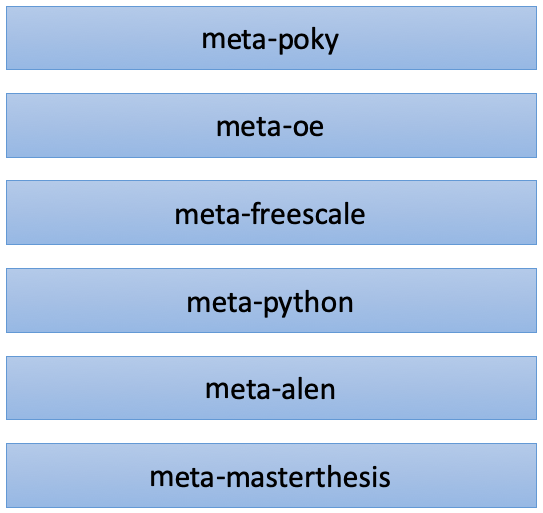
\includegraphics[width=.4\textwidth]{images/yocto_layer.png}
	\caption{\textit{Yocto Layer}}
	\label{fig:yocto_layer}
\end{figure}

\subsection{Verkabelung im Fahrzeug}

Damit die ALEN Zugriff auf den CAN-Bus bekommt, muss sie an ihn angeschlossen werden. Hierfür kommt prinzipiell jede beliebige Stelle der Linie im Auto infrage. Zum Beispiel kann dazu das CAN-Gateway angezapft werden oder ein T-Stück an den zwei Kabeln irgendwo in der Nähe des Fahrerraums. Hinter dem Lenkrad ist deshalb eine sehr gute Position, da es mit dem Antriebsstrang verbunden ist und viel Platz für die Montage bietet. Der Kabelbaum wird daher aufgetrennt und jeweils eine abzweigende Leitung an den CAN-High und CAN-Low gelötet. Bevor diese in eine RJ11 Buchse gesteckt werden, müssen sie gegen Reflexionen mit einem 120\si{\ohm} Widerstand terminiert werden. Für die Spannungsversorgung wird der 12V Zigarettenanzünder mit einem Adapter verwendet. Abbildung \ref{fig:alen_wireing} zeigt den schematischen Aufbau.

\begin{figure}[htbp]
	\centering
    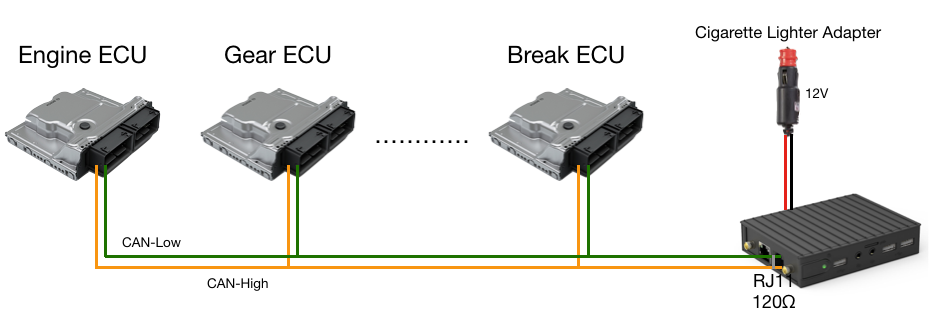
\includegraphics[width=.6\textwidth]{images/alen_wireing.png}
	\caption{ALEN Verkabelung}
	\label{fig:alen_wireing}
\end{figure}

\section{Softwarekomponenten}
\label{sec:software_compontens}

Die Architektur des Systems zeigt bereits auf, welche Softwarekomponenten auf der CCU zu realisieren sind. Diese sind in der folgenden Liste angeführt und in weiterer Folge im Detail erklärt.

\begin{enumerate}
    \item \textbf{CAN-Logger} zeichnet CAN-Nachrichten der Fahrwerks-CAN-Linie in fast-Echtzeit auf und speichert sie in MDF-Dateien ab.
    \item \textbf{Data-Preprocessor} bereitet die Daten für das \textit{Machine Learning} Model auf und speichert sie in HDF5-Dateien ab.
    \item \textbf{ML-Model Trainer} erstellt ein \textit{Machine Learning} Model mit einem \textit{Random Forest Classifier} und trainiert es mit den abgespeicherten Fahrerprofilen.
    \item \textbf{ML-Model Predictor} nimmt neue CAN-Dateien entgegen und klassifiziert die Datenpunkte mit dem ML-Model.
    \item \textbf{Result Presenter} sendet eine Benachrichtigung an den Fahrzeughalter, wenn eine gewisse Genauigkeit bei ausreichend Datenpunkten erzielt wird.
\end{enumerate}

\subsection{CAN-Logger}
\label{sec:can_logger}

Der Eintrittspunkt vom Fahrzeug zur ALEN ist über die CAN Schnittstelle. Bevor die CAN-Daten überhaupt verarbeitet werden können, muss es dem Betriebssystem möglich sein am Bus teilnehmen zu können. Es braucht auf der Netzwerkebene ein Interface und darüberliegend einen Treiber. Dies wird vom Kernel über das \textit{SocketCAN} Modul bereitgestellt \cite{kleine2012}. Es ist eine \textit{Open-Source} Sammlung aus einer Implementierung des CAN-Protokolls, Linux Treiber und einer CAN-Socket API. Das ermöglicht eine ähnliche Handhabung wie mit dem TCP/IP Protokoll-Stack, sodass sich Anwendungen gewöhnlich auf ein CAN-Interface mit einem Socket verbinden und Nachrichten empfangen, sowie senden können.

So verfährt auch der \textit{CAN-Logger}, dessen Aufgabe es ist, relevante Nachrichten vom Bus mitzulesen und abzuspeichern. Die Software ist in der Programmiersprache \textit{Go} entwickelt, da von \textit{Bosch} einige Bibliotheken für das Aufzeichnen und Verarbeiten von CAN-Daten für Linux-Systeme existieren. Durch eine Socketverbindung auf das CAN-Interface wird jede einzelne Botschaft als \textit{Raw Dataframe} eingelesen. Erst durch den Abgleich des \textit{Message Identifiers} mit der abgelegten CAN-Matrix kann die Nachricht interpretiert werden. Die Umrechnung der Werte in den dazugehörigen physikalischen Größen wird von einer \textit{Library} mithilfe der Spezifikationen von der DBC-Datei erledigt. Aus Performancegründen werden nicht alle Nachrichten von der CAN-Linie verarbeitet. In der Datenbank sind nur jene inkludiert, die für diese Anwendung relevant sind. Die originale Datei beinhaltet nämlich für den Antriebsstrang etwa 270 Nachrichten mit 1500 Signalen. Dies gilt konkret für einen VW Golf 7, jedoch unterscheidet es sich kaum zu anderen Fahrzeugtypen. Die tatsächlichen relevanten Signale können aus den Erkenntnissen des vorherigen Kapitels entnommen werden. Das Resultat der \textit{Feature Selection} aus \ref{sec:feature_selection} hat gezeigt, dass nur 21 \textit{Features} für ein aussagekräftiges ML-Ergebnis ausreichend sind. Welche das sind, sind in der Abbildung \ref{fig:feature_perm_importance} ersichtlich. Diese sind aus den folgenden acht Signalen errechnet und in sechs CAN-Botschaften enthalten.

\textit{Bremsdruck}, \textit{Geschwindigkeit}, \textit{Motordrehzahl}, \textit{Fahrpedalrohwert}, \textit{Längsbeschleunigung}, \textit{Querbeschleunigung}, \textit{Lenkradwinkel}, \textit{Lenkradgeschwindigkeit}

Die DBC-Datei wird demnach auf ein minimales Subset reduziert. Neben dem angesprochenen geringeren Rechenaufwand für den \textit{CAN-Logger} selbst, sinkt der notwendige Speicherbedarf und auch die darauffolgenden SW-Komponenten werden entlastet. Sie müssen nur die Signale verarbeiten, welche für die \textit{Machine Learning} Anwendung sinnvoll sind. Beim Erhalt einer CAN-Nachricht legt die Software die umgerechneten Werte mit einem in Nanosekunden aufgelösten Zeitstempel in den Speicher ab und nach jeweils einer Minute werden alle gesammelten Daten in eine MDF-Datei gespeichert.

\subsection{Data-Preprocessor}
\label{sec:data_preprocessor}

Das Resultat dieser Komponente sollen Daten sein, die direkt für das \textit{Machine Learning Model} verwertbar sind. Das bedeutet, dass sie das gleiche Format und die Struktur haben müssen, wie jene mit denen das \textit{Model} trainiert wurde. Da für den RF-Algorithmus durch das 4. Kapitel bereits optimale Parameter mit den vorhanden Datensätzen bekannt sind, werden die neuen Daten auf die gleiche Struktur gebracht. Des weiteren wird ebenfalls \textit{Python} mit den verwendeten Modulen eingesetzt.

Hierfür überwacht der \textit{Data-Preprocessor} das Verzeichnis in dem der \textit{CAN-Logger} die Dateien abspeichert und wenn eine neue hinzukommt, wird sie eingelesen. Der erste Schritt ist, die Frequenzen aller Signale anzugleichen. Wie in Abschnitt \ref{sec:data_preprocessing} beschrieben beträgt sie 0.5Hz. Danach gilt es die gewünschten 21 \textit{Features} aus den Signalen zu bekommen. Je nach Signal werden Minimal-, Maximal-, Durchschnittswert, Standardabweichung und Median berechnet. Der nächste Schritt löscht alle Datenreihen, wo sich das Auto im Stillstand, zum Beispiel bei einer roten Ampel, befindet. Diese Daten können nichts zur Klassifizierung beitragen, da sie keine Aussagekraft haben. Als letztes erfolgt das Speichern der neuen Datensätze in HDF5 Dateien.

\subsection{ML-Model Trainer}
\label{sec:ml_model_trainer}

Der \textit{ML-Model Trainer} ist die erste Softwareinstanz, welche nach dem Hochfahren der ALEN gestartet wird. Die Funktion dessen ist, einen \textit{Random Forest Classifier} zu erstellen und mit abgelegten Fahrerprofilen zu trainieren. Auch hier kommt \textit{Scikit-Learn} zum Einsatz und die Parameter werden wie erwähnt von den Optimierungsresultaten übernommen. Die Profile sind durch den \textit{CAN-Logger} aufgezeichnete und vom \textit{Data-Preprocessor} gefilterte Daten von jeweils einer Person. Dadurch ist sichergestellt, dass sie die gleichen Eigenschaften wie die zu klassifizierenden Daten haben und zu 100\% zuordenbar sind.

\subsection{ML-Model Predictor}
\label{sec:ml_model_predictor}

Nach dem \textit{Data-Preprocessor} ist der \textit{ML-Model Predictor} geschaltet. Er überwacht wiederum das Verzeichnis, indem die HDF5 Dateien nach der Vorverarbeitung gespeichert werden. Kommt eine neue Messdatei hinzu, wird sie eingelesen und auf ihre Korrektheit validiert. Darunter zählt die Überprüfung, ob alle Datenreihen inkludiert sind und ob alle Signale zu jedem gegebenen Zeitpunkt einen Wert haben. Ergeben sich Inkonsistenzen, wird die Datei übersprungen. So wird vermieden, dass es zu Verfälschungen während der Analyse kommt und dadurch auch zu keiner Missklassifizierung. Hat die Datei die erwartete Struktur, wird sie zu den in dieser gestarteten Fahrt bereits aufgenommen Daten hinzugefügt und in das erstellte Ml-Modell eingespeist. Das Ergebnis ist eine Reihe an Werten, welche jeweils die prognostizierte Klasse sind. Die Einträge repräsentieren somit den klassifizierten Fahrer für die entsprechende Eingabe-Datenreihe. Der nächste Schritt ist die Auswertung, um welche Fahrerin es sich dabei handelt. Als erstes wird die Häufigkeit der vorhandenen Klassen (1 bis 4) ermittelt. Danach können mehrere Methoden zur Evaluierung eingesetzt werden.

\subsubsection{Grenzwert}

Eine Möglichkeit ist folgende. Übersteigt der prozentuale Anteil eines Fahrers eine gewisse Grenze, ist mit dieser Wahrscheinlichkeit das der Fahrer. Zum Beispiel sind nach fünf Minuten Fahrzeit 150 Datenreihen (30 pro Minute, 0,5Hz) verfügbar. Das Resultat des \textit{Random Forest Models} hat ergeben, dass etwa sieben Messpunkte (5\%) zu Fahrer \textit{1} gehören könnten, 15 (10\%) zu Fahrer \textit{2} und über 22 (15\%) zum Fahrprofil \textit{3}. 105 (70\%) Eingabedaten deuten jedoch auf Fahrer \textit{4} hin. Muss die Grenze von 70\% erreicht werden, um eine Fahrer identifizieren zu können, würde das Endergebnis der Klassifizierung diesen Fahrer bevorzugen.

\subsubsection{Differenz}
\label{sec:identification_difference}

Angenommen der \textit{Output} des Modells ist nicht so eindeutig und ergibt jeweils für Fahrerin \textit{1} und \textit{2} 5\%, für Fahrerin \textit{2} 30\% und 60\% für Fahrerin \textit{4}. Nach dem ersten Ansatz wäre hier keine eindeutige Identifikation möglich. Um trotzdem auf ein zuverlässiges Ergebnis zu kommen, kann eine andere Herangehensweise angewendet werden. Sie betrachtet nur die zwei am häufigsten vorkommenden Klassen - in diesem Fall Fahrerin \textit{3} und \textit{4} - und bildet davon die Differenz. Ist diese groß genug, kann es für eine ausreichende Identifikation genügen. Hier bietet sich der Wert 30 an (Kriterium 1). Dadurch ist auch sichergestellt, dass die Klasse mit dem höchsten Anteil mindestens 50\% hat (Kriterium 2). Für ein besseres Verständnis sind unten Beispiele angeführt, welche alle für die Fahrerin \textit{4} sprechen.

\begin{table*}[htbp]
    \centering
    \caption{Beispiel Differenzansatz für Fahrerin 1 - 4}
    \label{tab:differencial_approach}
    \begin{tabular}{|l|l|l|l|l||l|l|l|}
        \hline
         & \textit{P(1)} & \textit{P(2)} & \textit{P(3)} & \textit{P(4)} & Kriterium 1 & Kriterium 2 & Ergebnis \\
        \hline
        1. min & 0\% & 0\% & 30\% & 70\% & 70 - 30 $\geq$ 30 & 70 $\geq$ 50 & \textit{P(4)} \\
        2. min & 10\% & 20\% & 10\% & 60\% & 60 - 20 $\geq$ 30 & 60 $\geq$ 50 & \textit{P(4)} \\
        3. min & 20\% & 20\% & 20\% & 50\% & 50 - 20 $\geq$ 30 & 50 $\geq$ 50 & \textit{P(4)} \\
        4. min & 10\% & 10\% & 30\% & 60\% & 60 - 30 $\geq$ 30 & 60 $\geq$ 50 & \textit{P(4)} \\
        5. min & 0\% & 10\% & 20\% & 75\% & 75 - 20 $\geq$ 30 & 75 $\geq$ 50 & \textit{P(4)} \\
        \hline
  \end{tabular}
\end{table*}

\subsubsection{Zeitliche Veränderung}

Weiters kann auch die zeitliche Veränderung der Häufigkeiten analysiert werden. Das ist hilfreich, wenn sich die Individualität der Personen erst nach den ersten Fahrminuten für das ML-Modell sichtbar macht. So müssen nicht mehr Daten als nötig gesammelt werden, um die nicht-eindeutigen zu kompensieren. Die Methode analysiert jede Datei für sich und speichert die Zwischenergebnisse ab. Danach wird jeweils das Delta berechnet und der Maximalwert bestimmt. Ist das Delta positiv und übersteigt sowie der Maximalwert eine gewisse Grenze, kann der Lenker identifiziert werden. Die Tabelle \ref{tab:time_dependet_analyzis} zeigt ein Beispiel, bei dem die ersten beiden Ansätze noch keinen Fahrer eindeutig identifizieren könnten. Im Durchschnitt sind 45\% der Daten auf Fahrer \textit{4} klassifiziert worden, was zu wenig ist. Die zeitbasierte Veränderung spricht jedoch klar dafür.

\begin{table*}[htbp]
    \centering
    \caption{Beispiel Zeitliche Veränderung der Wahrscheinlichkeiten für Fahrer 1 - 4}
    \label{tab:time_dependet_analyzis}
    \begin{tabular}{|l|l|l|l|l|}
        \hline
         & \textit{P(1)} & \textit{P(2)} & \textit{P(3)} & \textit{P(4)} \\
        \hline
        1. min & 20\% & 20\% & 30\% & 30\% \\
        2. min & 20\% & 25\% & 25\% & 30\% \\
        3. min & 10\% & 20\% & 30\% & 40\% \\
        4. min & 0\% & 20\% & 25\% & 55\% \\
        5. min & 0\% & 10\% & 20\% & 75\% \\
        \hline
        $\diameter$ & 10\% & 18\% & 26\% & 45\% \\
        \hline
        $\Delta$ & -20\% & -10\% & -15\% & +45\% \\
        \hline
        max & 20\% & 25\% & 30\% & 75\% \\
        \hline
  \end{tabular}
\end{table*}

Um eine Methode auswählen zu können, welche letztendlich für das System zum Einsatz kommt, wurde jede implementiert und mit den Testdaten mehrmals evaluiert. Das hat ergeben, dass sich der zweite Ansatz am besten hierfür eignet. Im Gegensatz zum ersten ist er flexibler und findet schneller den korrekten Fahrerin. Zusätzlich hat sich herausgestellt, dass bereits nach den ersten Minuten das Fahrverhalten der Testfahrer unterscheidbar ist. Daher ist die letzte Implementierung nicht anwendbar, da sich das Delta nicht merklich verändert. Als Absicherung kann des Weiteren die Anwendung so konfiguriert werden, dass die identifizierte Fahrerin erst dann bestätigt ist, wenn sich das Ergebnis bei den darauffolgenden Durchläufen nicht mehr ändert. Umso länger abgewartet wird, desto sicherer gilt es, aber umso länger muss mit der darauf basierenden Aktion gewartet werden. Es gilt daher das richtige Verhältnis zwischen der Identifikationszeit und wie lang auf die Umsetzung der Aktion gewartet werden darf, zu finden. Beispielsweise macht es für individuelle Anpassungen keinen Sinn länger als zehn Minuten zu warten, aber der Eintrag ins digitale Fahrtenbuch kann auch erst am Ende der Fahrt erfolgen.

\subsection{Result Presenter}

Wie die Aktion nun ausgelöst wird, übernimmt die Komponente \textit{Result Presenter}. Je nach Service kann dies auf unterschiedlichen Kommunikationswegen geschehen. Soll das Auto selbst darauf reagieren, zum Beispiel das Anzeigen der zuletzt ausgewählten Ziele im Navigationssystem, kann die Information wieder zurück über den CAN-Bus übertragen werden. Wird hingegen nach einer gewissen Zeit gar kein Fahrer erkannt, womöglich also eine unautorisierte Person, ist es denkbar eine SMS an den Fahrzeughalter zu versenden. Da die ALEN ein GSM Modul mit SIM-Karte integriert hat, ist es ohne weiteres umsetzbar. Über die Internetverbindung können auch Dienste des Herstellers oder von Drittanbietern angebunden werden, welche ein REST API zur Verfügung stellen. Es hängt demnach sehr stark davon ab, was mit der Erkenntnis passieren soll.

\subsection{Sequenzdiagramm}

Das folgende Diagramm (Abbildung \ref{fig:sw_components_sequence}) zeigt die Funktionen der einzelnen Komponenten. Dadurch, dass fast kein tatsächlicher Nachrichtenaustausch stattfindet, sondern meist nur Dateien abgelegt werden, gibt es wenige direkte Querverbindungen. Nach dem Hochfahren der ALEN, was in etwa zehn Sekunden dauert, wird zuerst der \textit{CAN-Logger} und der \textit{ML-Model Trainer} gestartet. Danach folgt der \textit{Data-Preprocessor}, der \textit{ML-Model Predictor} und der \textit{Result Presenter}. Obwohl es aus logischer Sicht unabhängige und alleinstehende Komponenten sind, werden die letzten drei bei der Umsetzung zusammengeführt. Das hat den Grund, dass einerseits die Klassifizierungslogik das zuvor erstellte Modell benötigt und andererseits unmittelbar danach die Funktion zum Weiterleiten der Information, welche kein großes Ausmaß annimmt, aufgerufen wird.

\begin{figure}[htbp]
	\centering
    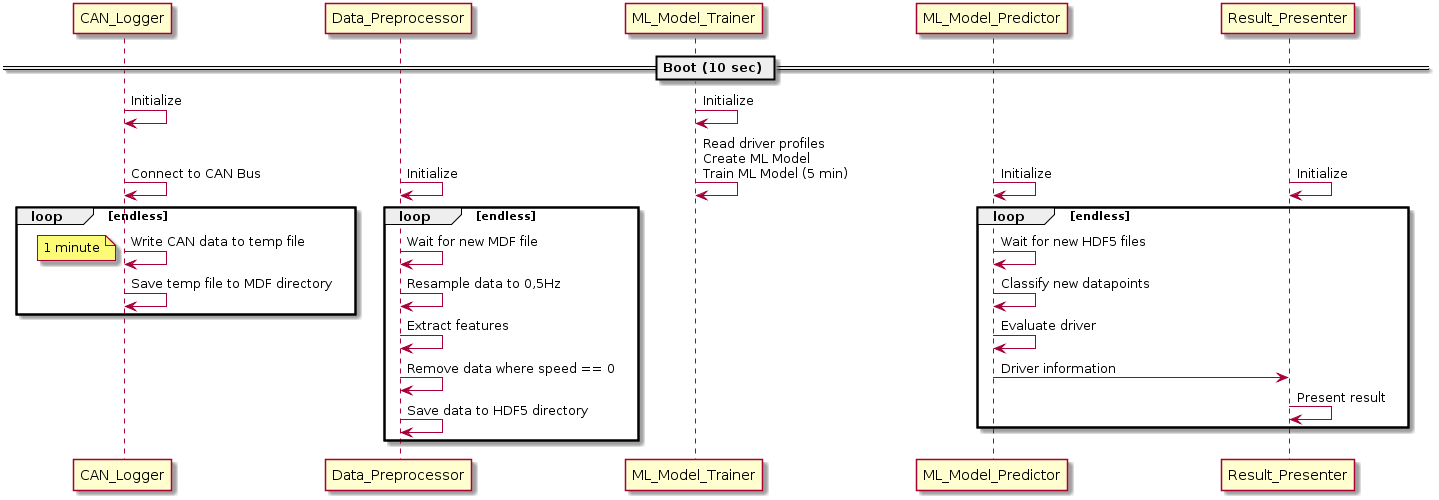
\includegraphics[width=\textwidth]{images/sw_components_sequence.png}
	\caption{Sequenzdiagramm Software Komponenten}
	\label{fig:sw_components_sequence}
\end{figure}

\section{Simulation}
\label{sec:simulation}

Das letzte Ziel der Masterarbeit ist, das entwickelte System in ein Fahrzeug zu integrieren. Da jedoch das Unternehmen, mit dem es umgesetzt wird, leider kein entsprechendes bereitstellen kann, muss es simuliert werden. Normalerweise würden vier Personen mehrere Testfahrten durchführen, um ein Profil anzulegen. Bei weiteren Fahrten könnte das System in Folge dessen erprobt werden. Da dies eben nicht möglich ist, dienen hierzu zufällige vier der vorhandenen Datensätze. Für diesen Zweck werden die Start- und Endzeitpunkte jeder Fahrt extrahiert und abgespeichert. Im Durchschnitt enthält ein Datensatz 46 Fahrten, von dem per Zufall zehn Fahrten entnommen werden, sodass diese nicht mehr in der originalen Datei enthalten sind. Das ist insofern wichtig, damit der \textit{Random Forest Classifier} die Testdaten nicht kennt und das Ergebnis verfälscht. Nach diesem Vorgang existiert daher pro Fahrer ein Trainingsset aus ungefähr 36 Fahrten und ein Testset aus zehn. Werden die Daten für einen Test, wie er zum Beispiel in Abschnitt \ref{chap:set_up} oder \ref{chap:optimization} gemacht wurde, verwendet, kommt eine Genauigkeit des Modells von ca. 94\% heraus. Die Steigerung erklärt sich durch die geringere Anzahl an Fahrerprofilen.

Um die Simulation so realgetreu wie möglich zu implementieren, wird nur der \textit{CAN-Logger} ersetzt. Stattdessen werden von einem eigenen Programm (\textit{MDF-Simulator}) MDF Dateien in das Verzeichnis abgelegt, aus dem der \textit{Data-Preprocessor} diese bezieht. Bei den MDF Dateien handelt es sich um jene, welche im \ref{chap:set_up}. Kapitel vorgestellt wurden und bilden das Testset. Da sie jeweils eine Minute an Fahrtzeit beinhalten, wird auch immer eine Datei nach einer Minute in das dezidierte Verzeichnis hinzugefügt. Die Reihenfolge ist dabei chronologisch, beginnend mit der ersten Minute einer Fahrt. Durch die neue Komponente wird lediglich das erste Glied (CAN-Bus und -\textit{Logger}) simuliert. Für die restlichen Software-Teile hat es keine Auswirkung. Da das ganze System auch auf der ALEN in Betrieb genommen wird, ergeben sich fast reale Bedingungen und die daraus resultierenden Ergebnisse haben eine hohe Aussagekraft.

Zusammenfassend lässt sich die Simulationsumgebung folgendermaßen beschreiben: Die Softwarekomponenten werden wie beschrieben implementiert, lediglich der \textit{CAN-Logger} wird durch den \textit{MDF-Simulator} ersetzt. Für die Identifikation eines Lenkers kommt der \textit{Differenz}-Ansatz um Einsatz. Als Fahrerprofile werden vier der vorhandenen Datensätze herangezogen, bei denen zehn Fahrten gelöscht werden. Die original MDF Dateien von den gelöschten dienen hierzu als Eingabedaten. Bei einem Testdurchlauf verwendet der \textit{MDF-Simulator} immer nur Dateien von einer Fahrerin, da es darum geht, nur einen zu identifizieren. Zur Benachrichtigung wird ein SMS-Versand mit dem integrierten Modul und SIM-Karte umgesetzt.

\subsection{Fahrererkennung}
\label{sec:driver_identification}

Das Listing \ref{lst:sw_rf} zeigt einen Ausschnitt der letzten drei genannten Komponenten. Von Zeile zwei bis elf werden die abgelegten Fahrerprofile geladen, ein \textit{Random Forest Classifier} erstellt und trainiert. Ab Zeile dreizehn beginnt die Logik für die Fahrererkennung. Es beinhaltet das Einlesen neuer Messdaten sowie die Klassifizierung durch das ML-Modell. Danach werden die Häufigkeiten der Klassen gezählt und die zwei am meisten vorkommenden ermittelt. Anschließend wird die Überprüfung nach dem \textit{Differenz}-Ansatz durchgeführt und schlussendlich eine SMS Versand, wenn der Fahrer oft genug bestätigt wurde.

\begin{lstlisting}[frame=lines, caption=Ausschnitt Fahreridentifikation, captionpos=b, label = lst:sw_rf, numbers=left, language=Python, showstringspaces=false, basicstyle=\footnotesize]
    [...]
    # ML Model Trainer
    profiles = get_profiles(config["profile_dir"])
    features = config["features"][:21]
    X = profiles[features].values
    Y = profiles["class"]

    clf = RandomForestClassifier(n_estimators=300, min_samples_leaf=1, min_samples_split=3, criterion="gini", max_depth=None)
    clf.fit(X, Y)

    # ML-Model Predictor
    all_data = []
    while True:
        data = []
        for file in os.listdir(config["input_dir"]):
            df = pd.read_hdf(os.path.join(config["input_dir"], file))
            data.append(df)

        all_data = all_data + data

        pdata = pd.concat(all_data, sort=False)
        pdata = pdata.values

        pred = clf.predict(pdata)

        ids, counts = np.unique(pred, return_counts=True)
        ids = dict(zip(ids, counts))
        first = {"id": None, "count": 0}
        second = {"id": None, "count": 0}
        for id in t:
            c = ids[id]
            if c > first["count"]:
                first["count"] = c
                first["id"] = id
            elif c > second["count"]:
                second["count"] = c
                second["id"] = id

        first_conf = first["count"] / len(pred)
        second_conf = second["count"] / len(pred)
        diff = first_conf - second_conf
        if diff >= 0.30 and first_conf >= 0.50:
            if confirmed_id == first["id"]:
                confirmation_count += 1
            else:
                confirmed_id = first["id"]
                confirmation_count = 1

        if confirmation_count == config["confirmation_count"]:
            # Result Presenter
            send_SMS("\nDriver with id %s is driving" % first["id"], config["number"])
            break
    [...]
\end{lstlisting}

\subsection{Ergebnisse}

In diesem Abschnitt werden kurz die Ergebnisse der Simulation auf der ALEN präsentiert. Bis das \textit{Machine Learning Model} fertig trainiert ist, vergehen ca. fünf Minuten bei vier Profilen mit allen verfügbaren Fahrten (exklusive zehn). Aufgrund dessen beträgt die Anzahl wie oft eine Fahrerin hintereinander identifiziert werden muss fünf. Es liegen nämlich nachdem das Trainieren des Modells abgeschlossen ist, bereits fünf Dateien mit jeweils einer Minute an Fahrzeit vor. Für das Klassifizieren einer neuen Datei benötigt das Gerät unter eine Sekunde.

Bei einem Testdurchlauf wurde jeweils eine Fahrt herangezogen und festgestellt wie viele Minuten nötig sind, bis der Fahrer korrekt identifiziert wird. Um ein fundierteres Ergebnis zu bekommen, ist der Vorgang öfters mit permutierten Trainings- und Testfahrten durchlaufen worden. Der ganze Vorgang wurde auch mit allen vier Fahrern vollzogen. Dabei ist das Folgende herausgekommen.

\begin{itemize}
    \item Der Algorithmus hat mit einer Wahrscheinlichkeit von 97\% den Fahrer korrekt identifiziert.
    \item Lediglich drei Fahrten wurden falsch zugeordnet.
    \item Nur eine Fahrt konnte gar nicht zugeordnet werden.
    \item Für eine Identifikation wurden im Schnitt 5,73 Minuten an Fahrzeit benötigt.
\end{itemize}